\chapter{Introduction}
% HOW TO USE THESE FILES: each section lists, as comments, the points to cover and where the
% facts come from (repo docs). Write the text yourself under each heading, in your own words,
% and delete the [Write ...] placeholders and these comments as you go.

[Write 1--2 opening paragraphs: what PM2.5 is and why ground-level estimates matter.]

\section{Background}
% - PM2.5: particles <= 2.5 um; health effects (cite a WHO / health source you choose).
% - India's ground network: CPCB continuous stations; sparse outside cities.
%   Study area has 113 stations with valid data for 5 states (docs/stage2_acquisition.md).
% - Satellites see everywhere: aerosol optical depth (AOD, MAIAC) and trace gases (TROPOMI)
%   \cite{lyapustin2018maiac,veefkind2012tropomi}; reanalysis \cite{hersbach2020era5,gelaro2017merra2}.
[Write the background.]

\begin{figure}[h]
\centering
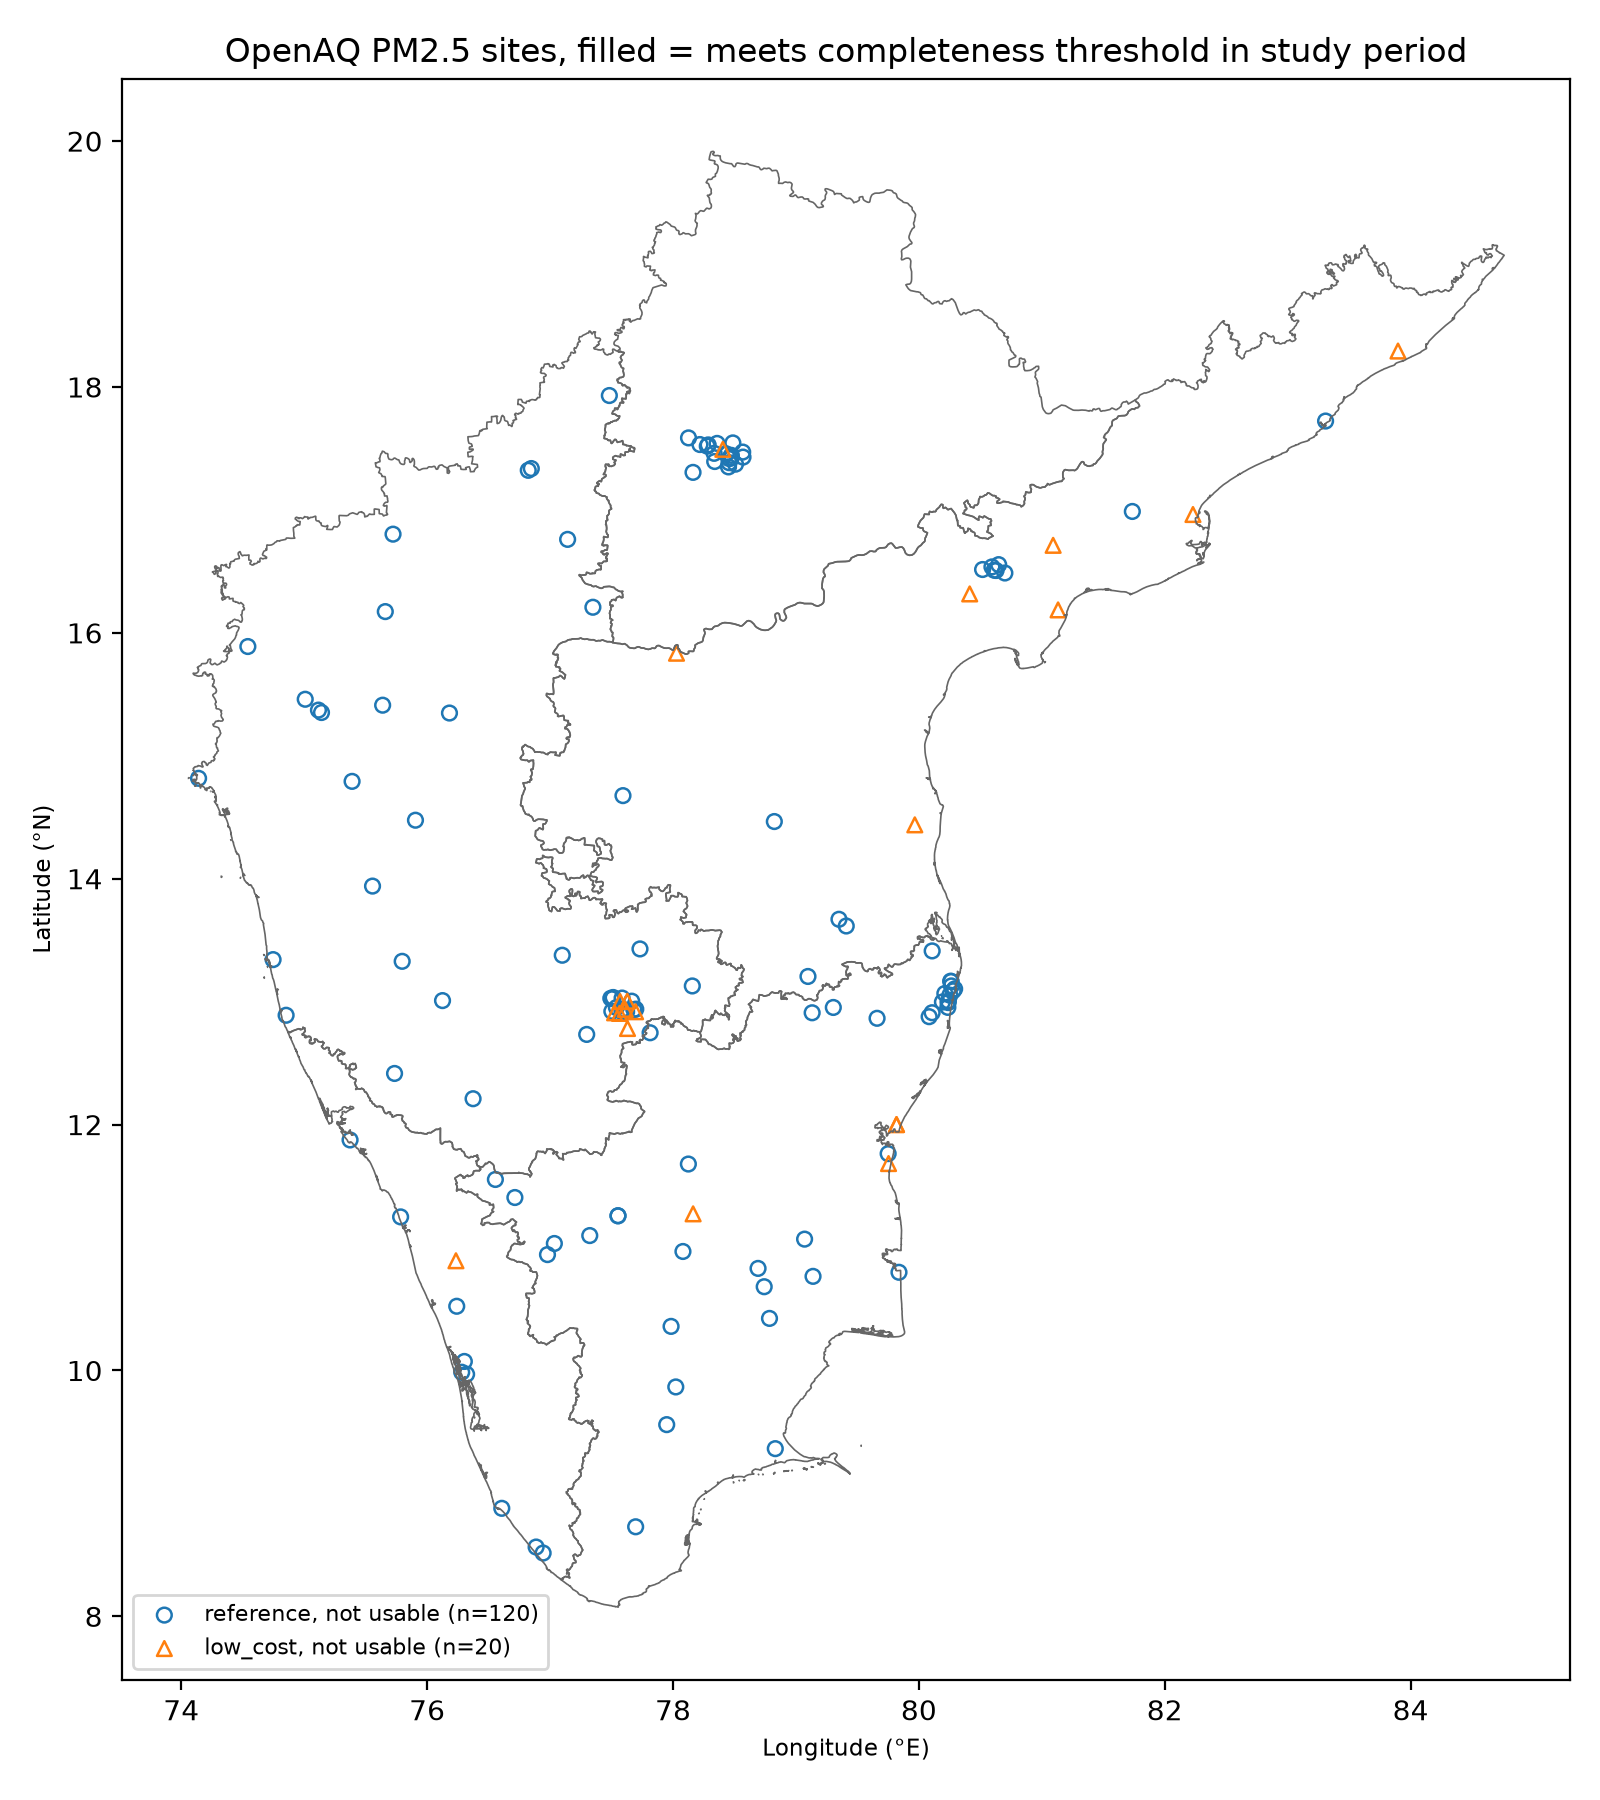
\includegraphics[width=11cm, height=8cm]{station_map}
\caption{Ground PM2.5 monitoring stations used in this study (CPCB and US Consulate monitors) over the five South Indian states.}
\label{fig:station_map}
\end{figure}
% Refer to it in the text as Figure~\ref{fig:station_map}.

\section{Motivation}
% - Satellites cannot see through cloud; South India has two monsoons.
% - Key fact: MAIAC AOD exists at the station pixel on 32.4 % of valid station-days, and in the
%   Kerala SW monsoon on about 1 day in 9 (docs/feasibility_summary.md, stage2_acquisition.md).
% - So any satellite-based model must work when the satellite is missing.
[Write the motivation.]

\section{Problem statement}
% One paragraph: how much do cloud and the monsoon degrade satellite-based PM2.5 estimation in
% South India, and how much does a two-tier model (with / without satellite inputs) recover?
[Write the problem statement.]

\section{Objectives}
% Suggested list (edit to your words):
% 1. Build a reproducible multi-source dataset (ground, satellite, reanalysis, static), 2021-2025.
% 2. Quantify satellite availability under cloud and by season.
% 3. Estimate daily PM2.5 with a two-tier model (Tier A with satellite, Tier B without) and
%    evaluate it at unmonitored stations (spatial cross-validation).
% 4. Measure the satellite gain overall, by cloud fraction and in the SW monsoon.
% 5. (Add-on) Forecast hourly PM2.5 1-72 h ahead at existing stations and compare with the literature.
\begin{enumerate}
  \item [Objective 1]
\end{enumerate}

\section{Scope}
% - Five states: Kerala, Karnataka, Tamil Nadu, Andhra Pradesh, Telangana (D010).
% - Period 2021-2025 (D011, D023); daily target, valid day >= 18 h (D012).
% - Station-level estimation in Phase 1; the 1 km grid map is Phase 2 (D026).
% - Out of scope: low-cost sensors (D015), road density (D033).
[Write the scope.]

\section{Organisation of the report}
% One short paragraph: what each chapter contains.
[Write the organisation.]
